%%%%%%%%%%%%%%%%%%%%%%%%%%%%%%%%%%%%%%%%%%%%%%%%%%%%%%%%%%%%%%%%
%                                                              %
%                                                              %
% Macallyster S. Edmondson                                     %
%                                                              %
% ECE351-53                                                     %
%                                                              %
% Lab #2                                                       %
%                                                              %
% 02/01/2022                                                   %
%                                                              %
% Straigtforward layout, broken into sections, uses many       %
% common libraries. Note, Hyperlinks are not highlighted.      %
%                                                              %
%%%%%%%%%%%%%%%%%%%%%%%%%%%%%%%%%%%%%%%%%%%%%%%%%%%%%%%%%%%%%%%%

%%%%%%%%%%%%%%%%%%%%%%%%%%%%%%%%%%%%%%%%%%%
%%% DOCUMENT PREAMBLE %%%
\documentclass[12pt]{report}
\usepackage[english]{babel}
%\usepackage{natbib}
\usepackage{url}
\usepackage[utf8x]{inputenc}
\usepackage{amsmath}
\usepackage{graphicx}
\graphicspath{{./images/}}
\usepackage{parskip}
\usepackage{fancyhdr}
\usepackage{vmargin}
\usepackage{listings}
\usepackage[hidelinks]{hyperref}
\usepackage{xcolor}
\usepackage{datetime}
\usepackage[section]{placeins}
\definecolor{codegreen}{rgb}{0,0.6,0}
\definecolor{codegray}{rgb}{0.5,0.5,0.5}
\definecolor{codeblue}{rgb}{0,0,0.95}
\definecolor{backcolour}{rgb}{0.95,0.95,0.92}
\lstdefinestyle{mystyle}{
backgroundcolor=\color{backcolour},
commentstyle=\color{codegreen},
keywordstyle=\color{codeblue},
numberstyle=\tiny\color{codegray},
stringstyle=\color{codegreen},
basicstyle=\ttfamily\footnotesize,
breakatwhitespace=false,
breaklines=true,
captionpos=b,
keepspaces=true,
numbers=left,
numbersep=5pt,
showspaces=false,
showstringspaces=false,
showtabs=false,
tabsize=2
}
\lstset{style=mystyle}
\setmarginsrb{3 cm}{2.5 cm}{3 cm}{2.5 cm}{1 cm}{1 cm}{1 cm}{1.5 cm}
\title{Lab \#2 Report}
% Title
\author{Macallyster S. Edmondson}
% Author
\date{\today}
% Date
\makeatletter
\let\thetitle\@title
\let\theauthor\@author
\let\thedate\@date
\makeatother
\pagestyle{fancy}
\fancyhf{}
\rhead{\theauthor}
\lhead{\thetitle}
\lfoot{Page: \thepage}
\rfoot{\thedate}
\fancypagestyle{customplain}{ %Used for default pages with plain style to keep overall document consistency
  \fancyhf{}
  \renewcommand{\headrulewidth}{0pt} %Remove bar from top of page
  \lfoot{Page: \thepage}
}
\fancypagestyle{titlepage}{ %Used for default pages with plain style to keep overall document consistency
  \fancyhf{}
  \renewcommand{\headrulewidth}{0pt} %Remove bar from top of page
  \cfoot{\thedate}
}
%%%%%%%%%%%%%%%%%%%%%%%%%%%%%%%%%%%%%%%%%%%%
\begin{document}
%%%%%%%%%%%%%%%%%%%%%%%%%%%%%%%%%%%%%%%%%%%%%%%%%%%%%%%%%%%%%%%%%%%%%%%%%%
%%%%%%%%%%%%%%%
\begin{titlepage}\thispagestyle{titlepage}
\centering
%\vspace*{0.5 cm}

\includegraphics[scale = 0.12]{univ-logo.png}\\[1.0 cm]
%University of Idaho
\begin{center}    \textsc{\Large   ECE 351 - Section \#53 }\\[2.0 cm]
\end{center}% University Name

%Lab Report
\rule{\linewidth}{0.2 mm} \\[0.4 cm]
{ \huge \bfseries \thetitle}\\
\rule{\linewidth}{0.2 mm} \\[0.5 cm]
\textsc{\Large User-Defined Functions }\\[1.5 cm] % Course 
\begin{minipage}{0.4\textwidth}
\begin{flushleft} \large
\emph{Submitted To:}\\
Kate Antonov\\ \small
University of Idaho\\
kantonov@uidaho.edu\\
\hfill
\end{flushleft}
\end{minipage}~
\begin{minipage}{0.4\textwidth}
\begin{flushright} \large
\emph{Submitted By :} \\
\theauthor \\ \small
University of Idaho\\
edmo7033@vandals.uidaho.edu\\
\href{http://github.com/mac-edmondson}{github.com/mac-edmondson}\\
\end{flushright}
\end{minipage}\\[2 cm]
\vfill
\end{titlepage}
%%%%%%%%%%%%%%%%%%%%%%%%%%%%%%%%%%%%%%%%%%%%%%%%%%%%%%%%%%%%%%%%%%%%%%%%%%
%%%%%%%%%%%%%%%
\tableofcontents\thispagestyle{customplain}
\pagebreak
%%%%%%%%%%%%%%%%%%%%%%%%%%%%%%%%%%%%%%%%%%%%%%%%%%%%%%%%%%%%%%%%%%%%%%%%%%
%%%%%%%%%%%%%%%
\renewcommand{\thesection}{\arabic{section}}
\section{Introduction}
The goal of this lab was to introduce the idea of user-defined functions in Python and utilize them to create causal functions we've learned about in \textbf{ECE 350}.
We then utilized these functions to demonstrate signal operations including time shifting, time scalin, time reversal, signal addition, and discrete-differentiation.
In order to complete this lab, the Python programming language was used with the \textit{Spyder-IDE} downloaded using \textit{Python Anaconda3}. The packages used in the 
completion of this lab were \texttt{numpy} for definitions of mathematical functions, and \texttt{matplotlib.pyplot} to plot outputs of functions seen later in this lab. 
All code for this lab, including this report, can be found on \href{http://github.com/mac-edmondson}{my Github}.
\section{Equations}
The equations used within this lab are shown in this section. The equations will be referenced by number throughout the rest of the report.
\begin{equation}\label{eq: 1}
  \begin{aligned}[c]
    u(t) = \left\{
      \begin{array}{ll}
        0 & \quad t < 0 \\
        1 & \quad t \geq 0
      \end{array}
    \right.\\
  \end{aligned}
\end{equation}
\begin{equation}\label{eq: 2}
  \begin{aligned}[c]
    r(t) = \left\{
      \begin{array}{ll}
        0 & \quad t < 0 \\
        t & \quad t \geq 0
      \end{array}
    \right.
  \end{aligned}
\end{equation}
\begin{equation}\label{eq: 3}
  \begin{aligned}
    y(t) = r(t) - r(t-3) + 5u(t-3) - 2u(t-6) - 2r(t-6)
  \end{aligned}
\end{equation}

\section{Methodology}
\subsection{Lab: Part 1}
In Part 1 of this lab, the goal was to implement $y=\cos{(t)}$ and plot the output based on the example code give in the lab handout. The main goal of this part 
was to find an optimal step size for good resolution curves. The code for this part of the lab can be seen below and the graph can be seen in Figure \ref{fig: p1t2}.
\begin{lstlisting}[language=Python, basicstyle=\footnotesize]
  # PART 1:

  def func1(t) :
      return np.cos(t)

  step_size = .1
  t = np.arange(0, 10 + step_size, step_size)
  y = func1(t)

  plt.subplot(1, 1, 1)
  plt.plot(t, y)
  plt.grid()
  plt.ylabel('cos(t)')
  plt.xlabel('t')
  plt.title('cos(t) v. t ; from 0 to 10, inclusive')
  plt.show()
\end{lstlisting}
\subsection{Lab: Part 2}
In Part 2 of this lab, the implementation of Equation \eqref{eq: 3} was the overall goal. Equation \eqref{eq: 3} was derived from a given graph in the lab handhout. In order to to
implement this equation, Equations \eqref{eq: 1} \& \eqref{eq: 2} needed to be defined in Python. Implementation of all three of the equations in Python can be seen in the source 
code below. (Code for plots is not shown to reduce report length. See Github for full code.) 
Each equation was implemented in it's own function, with the unit step function and ramp functions being defined with if-else statements. Then, the implementation of 
Equation \eqref{eq: 3} utilized both of those function definitions. The plots the code generates can be seen in Figures \ref{fig: p2t2} \& \ref{fig: p2t3}. As can be seen in those plots,
each function was working as expected.
\begin{lstlisting}[language=Python, basicstyle=\footnotesize]
  # PART 2:

  def u(t) :
      y = np.zeros(t.shape)
      
      for i in range(len(t)):
          if t[i] < 0 :
              y[i] = 0
          else:
              y[i] = 1
      
      return y

  def r(t) :
      y = np.zeros(t.shape)
      
      for i in range(len(t)):
          if t[i] < 0:
              y[i] = 0
          else:
              y[i] = t[i];

      return y

  def fig2_func(t) :
    y = r(t) - r(t-3) + 5 * u(t-3) - 2 * u(t-6) - 2*r(t - 6)
    return y
\end{lstlisting}
\subsection{Lab: Part 3}
In Section 3 of this lab, we used the function that implemented Equation \eqref{eq: 3} to perform time-shifting and scaling operations. Additionally, we took the discrete derivative
of the function using the \texttt{numpy.diff()} function. As seen in Figures \ref{fig: p3t1}, \ref{fig: p3t2}, \& \ref{fig: p3t3}, basic time reversal, time-shift, and time scaling 
operations were performed on Equation \eqref{eq: 3}, respectively, using Python. This was as simple writing it out by hand, just modifying the input to the defined function before
plotting it as seen in the code below.
\begin{lstlisting}[language=Python, basicstyle=\footnotesize]
  #PART 3:
  
  step_size = 1e-3

  #1
  t = np.arange(-10, 5 + step_size, step_size)
  y = fig2_func(-t)

  #2

  t = np.arange(-1, 14 + step_size, step_size)
  y = fig2_func(t-4)

  #3

  t = np.arange(-1, 10*2 + step_size, step_size)
  y = fig2_func(t/2)
\end{lstlisting}
Implementation of the discrete derivative was more complex. It is important to remember $y'(t) = \frac{\Delta y(t)}{\Delta t}$. Then, that derivative is still plotted against time.
Notice in the code below, t has to be shortened to the length of \texttt{dy} as there is one less value in the \texttt{dy} \& \texttt{dt} arrays from the \texttt{numpy.diff()} function. 
(Seek \texttt{numpy} documentation for more details.) Additionally, it is important to set the bounds of the y-axis using the \texttt{matplotlib.pyplot.ylim()} function, due to the 
very large rate of change from step functions in the discrete derivative. The plot of the discrete derivative can be found in Figure \ref{fig: p3t5}.
\begin{lstlisting}[language=Python, basicstyle=\footnotesize]
  #4

  t = np.arange(0, 10 + step_size, step_size)
  y = fig2_func(t)

  dt = np.diff(t, axis=0)
  dy = np.diff(y, axis =0)     
  
  plt.figure(figsize = (10, 7))
  plt.subplot(1, 1, 1)
  plt.plot(t[range(len(dy))], dy/dt)
  plt.ylim(-3, 10)
  #...
\end{lstlisting}
\section{Results}
The results of this lab are very straightforward. The implementation of all functions worked as expected and there is not much to discuss that wasn't covered in the Methodology 
Section of this report. 

It is important to note the difference in the discrete derivative of Equation \eqref{eq: 3} found using python, Figure \ref{fig: p3t5}, and the hand-drawn version of the same derivative, Figure \ref{fig: p3t4}. 
These derivatives look very similar but in the discrete derivative, there are large spikes in the rate-of-change where there are discontinuities in the hand-drawn plot. The reason
for this is that the discrete derivative does not have an \textit{absolute} instantaneous rate-of-change since there are a limited number of steps in \texttt{y}. With theoretical math, 
we know the rate of change is instantaneous at the points of discontinuity from Equation \eqref{eq: 1}. This being said, these large spikes in rate of change can be considerd as discontinuities.
\\
\begin{figure}[h!]
  \centering
  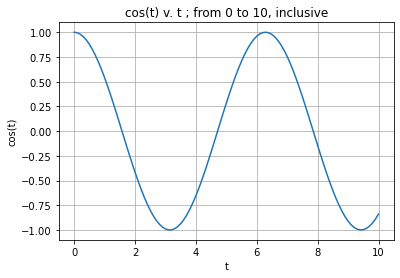
\includegraphics[scale=0.6]{p1t2.png}
  \caption{Part 1, Task 2 - Cosine Function Implementation}
  \label{fig: p1t2}
\end{figure}
\begin{figure}[h!]
  \centering
  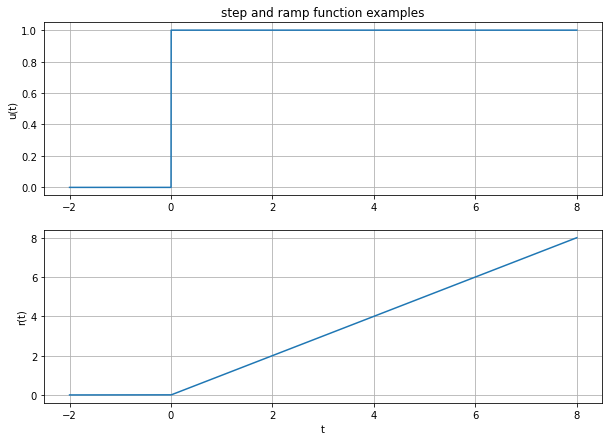
\includegraphics[scale=0.5]{p2t2.png}
  \caption{Part 2, Task 2 - Step and Ramp Function Implementation}
  \label{fig: p2t2}
\end{figure}
\begin{figure}[h!]
  \centering
  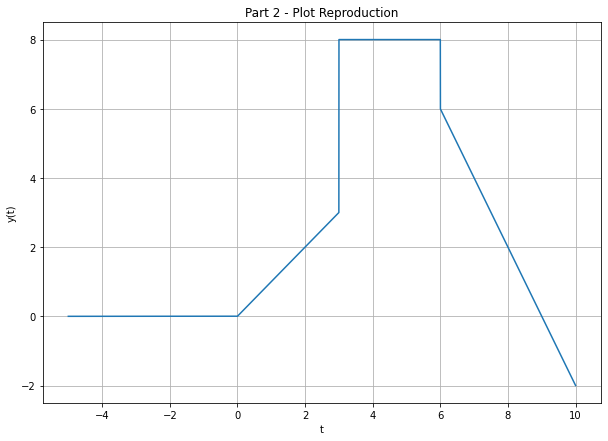
\includegraphics[scale=0.5]{p2t3.png}
  \caption{Part 2, Task 3 - Implementation of Equation \eqref{eq: 3}}
  \label{fig: p2t3}
\end{figure}
\begin{figure}[h!]
  \centering
  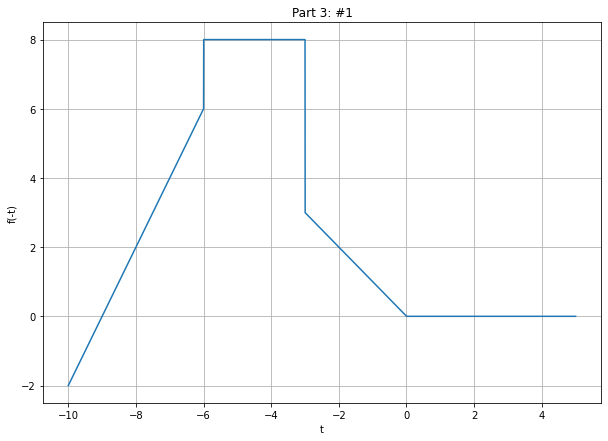
\includegraphics[scale=0.5]{p3t1.png}
  \caption{Part 3, Task 1 - Time Reversal Operations}
  \label{fig: p3t1}
\end{figure}
\begin{figure}[h!]
  \centering
  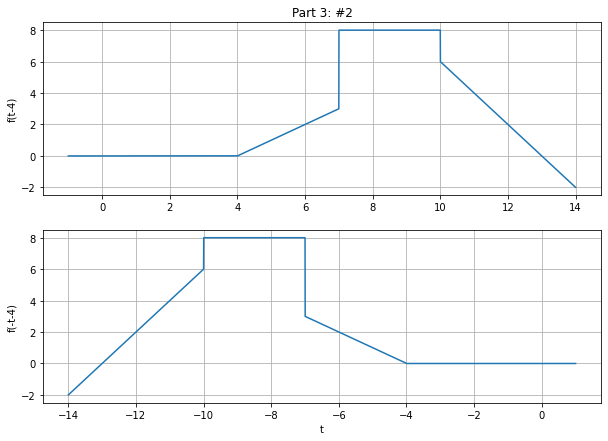
\includegraphics[scale=0.5]{p3t2.png}
  \caption{Part 3, Task 2 - Time-Shifting Operations}
  \label{fig: p3t2}
\end{figure}
\begin{figure}[h!]
  \centering
  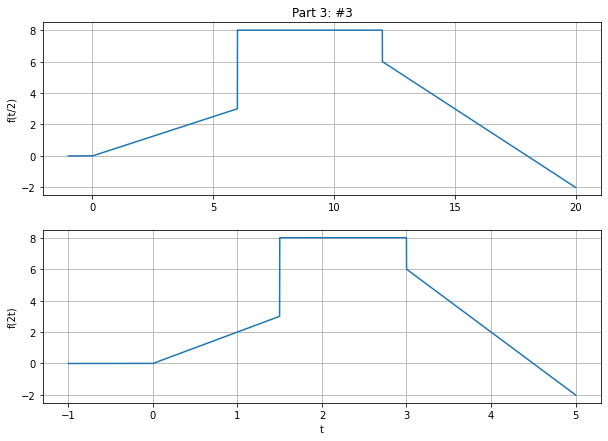
\includegraphics[scale=0.5]{p3t3.png}
  \caption{Part 3, Task 1 - Time Scaling Operation}
  \label{fig: p3t3}
\end{figure}
\begin{figure}[h!]
  \centering
  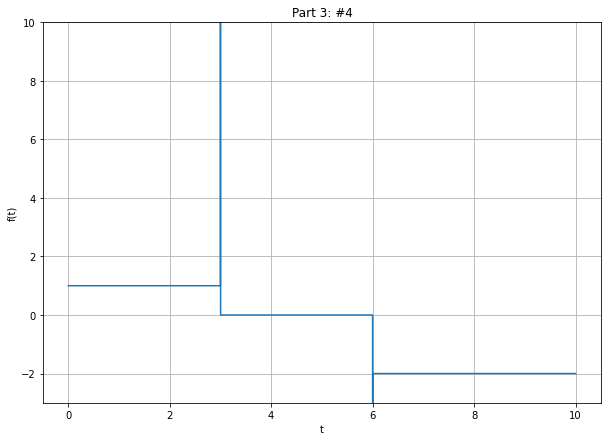
\includegraphics[scale=0.5]{p3t5.png}
  \caption{Part 3, Task 4 - Discrete Derivative of Equation \eqref{eq: 3}}
  \label{fig: p3t5}
\end{figure}
\begin{figure}[h!]
  \centering
  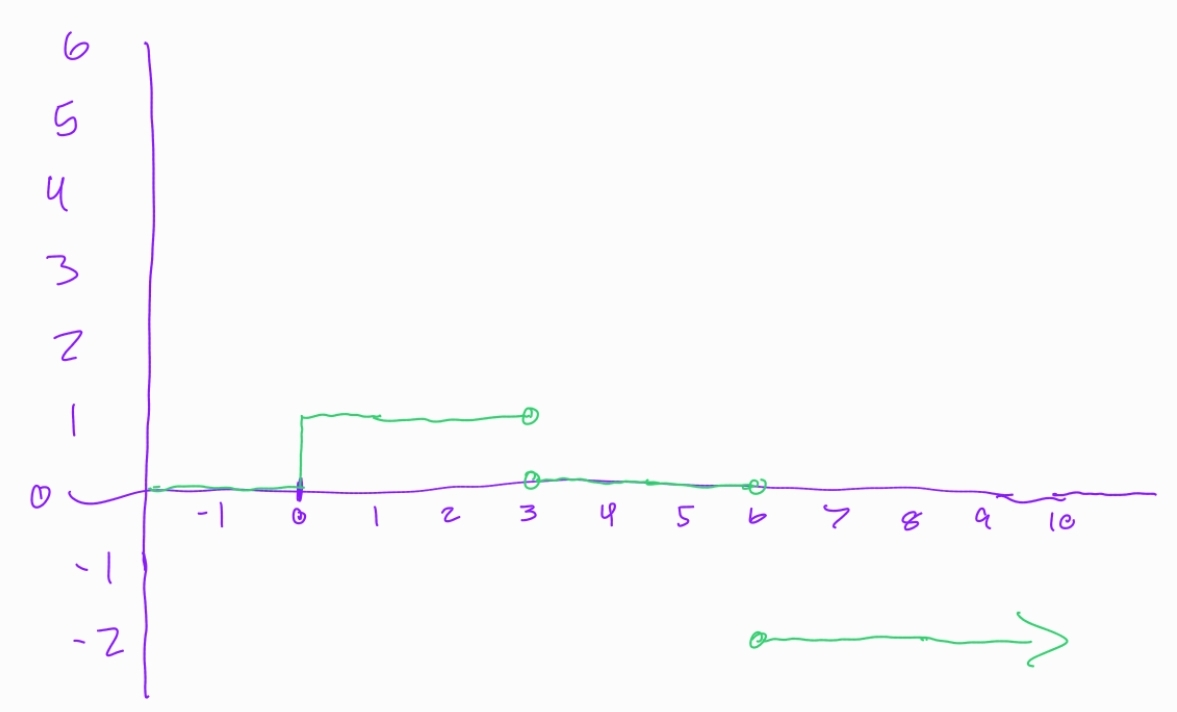
\includegraphics[scale=0.35]{p3t4.jpg}
  \caption{Part 3, Task 4 - Hand Drawn Derivative of Equation \eqref{eq: 3}}
  \label{fig: p3t4}
\end{figure}
\section{Error Analysis}
One problem that occurred during this lab which took up most of the lab time was figuring out how to take the discrete derivative of Equation \eqref{eq: 3}. This 
problem was solved by talking to the Lab TA, looking at the \texttt{numpy} documentation, and refering to the very important equation, $y'(t) = \frac{\Delta y(t)}{\Delta t}$. 
Other than this, I had no real issues.
\section{Questions}
\begin{itemize}
  \item See the second paragrah of Reports Section for the answer to this question.
  \item If the step size were changed for the discrete derivative of Equation \eqref{eq: 3} in Python, the main difference that would be seen in its plot would be larger magnitude
  spikes where the rate of change should be instantaneous. This is again due to the fact that there are a discrete amount of values in the output of the python functions.
  \item This lab was very clear and I had a lot of fun doing it. I have already used python to create plots for other classes and really enjoy it! All tasks, expectations, and 
  deliverables for this lab have been very clear. I do hope I get feedback on how to better organize my reports if the organization of this report is not up to standards.
\end{itemize}
\section{Conclusion}
In conclusion, I feel this lab was very successful. No doubt, this was a great introduction to plotting and defining functions in Python. I really enjoyed the discrete derivative 
that was performed with Python and I think this should be an introductary lab for all future semesters. I have no feedback on possible sources of improvement.
\newpage
\begin{thebibliography}{111}
\thispagestyle{customplain}

\end{thebibliography}
\end{document}
%This template was created by Roza Aceska.